\section{Evaluation}\label{sec:eval}
When running benchmarks we compile three versions of each benchmark: duplicating nothing, duplicating both inputs, and only duplicating one of the two inputs.
We discuss the specific performance tradeoffs of this choice.
\begin{figure*}
    \begin{subfigure}{0.3\textwidth}
        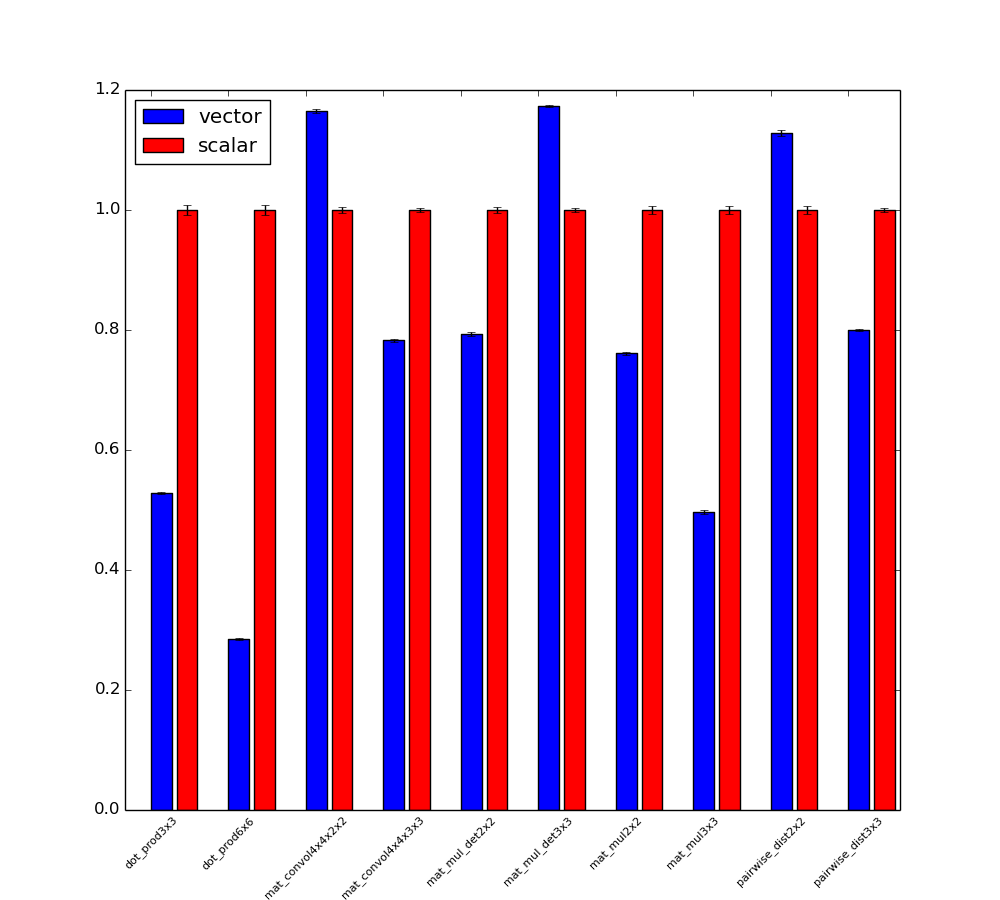
\includegraphics[width=0.95\textwidth]{figures/graphs/DataUnreplicatedENC+RUN.png}
        \caption{Scalar vs. Vector comparison for unreplicated inputs}
    \end{subfigure}
    \begin{subfigure}{0.3\textwidth}
        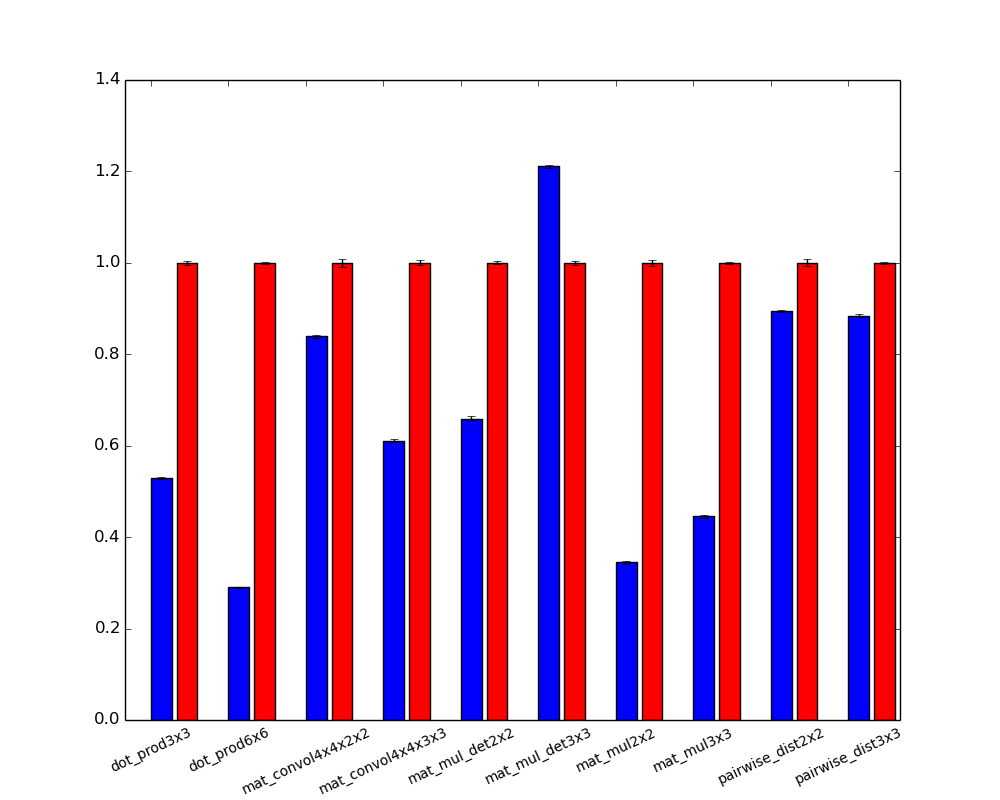
\includegraphics[width=0.95\textwidth]{figures/graphs/DataPartiallyReplicatedENC+RUN.png}
        \caption{Scalar vs. Vector comparison for partially replicated inputs}
    \end{subfigure}
    \begin{subfigure}{0.3\textwidth}
        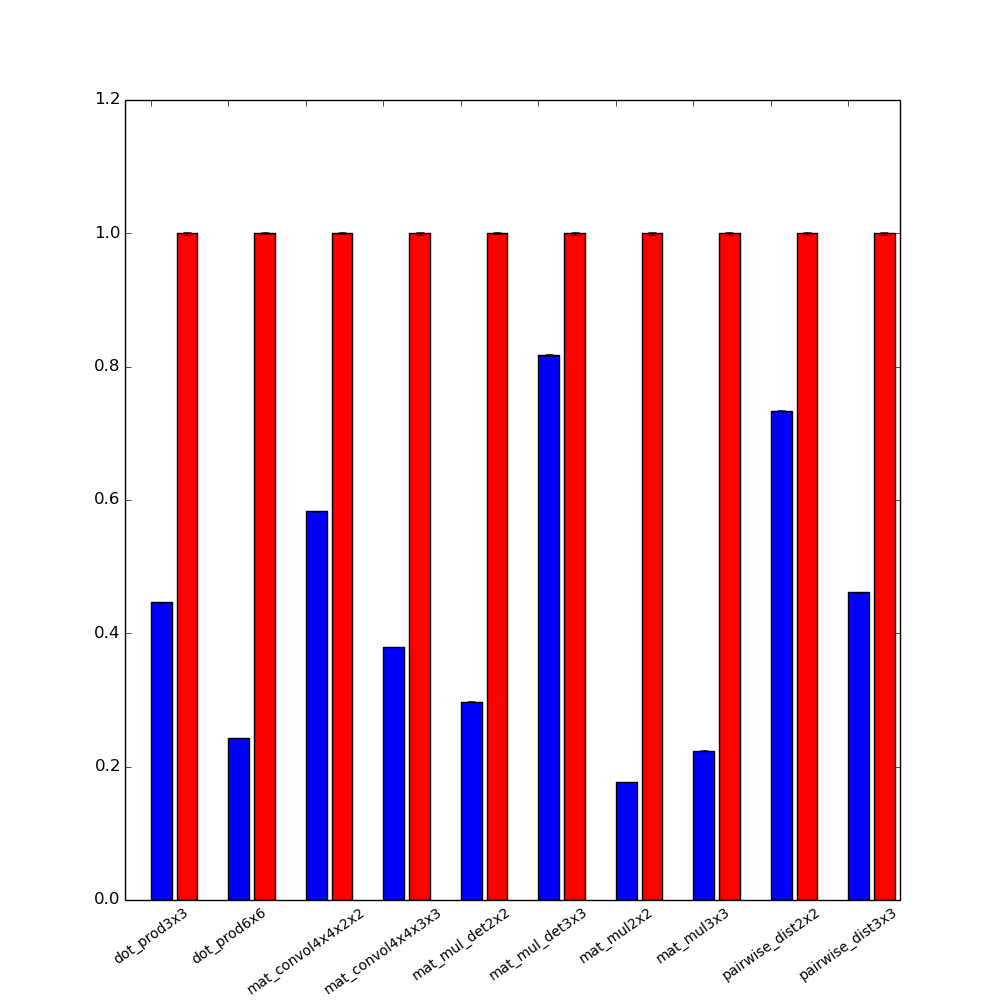
\includegraphics[width=0.95\textwidth]{figures/graphs/DataReplicatedENC+RUN.png}
        \caption{Scalar vs. Vector comparison for fully replicated inputs}
    \end{subfigure}
    \caption{Scalar vs. Vector encryption + run time comparisons for various replication regimes. Scalar run time is normalized to 1, so a smaller vector bar is better.}
\end{figure*}